\begin{flushright} {\tiny {\color{gray} \tt mms\_db3d.tex}} \end{flushright}
%~~~~~~~~~~~~~~~~~~~~~~~~~~~~~~~~~~~~~~~~~~~~~~~~~~~~~~~~~~~~~~~~~~~~~~~~~~~~~~~~~~~~~~~~~~~~~~~~~~

This benchmark begins by postulating a polynomial solution to the 3D Stokes equation 
as presented in \textcite{dobo04} (2004):
\begin{equation}
\vec{\upnu}
=
\left(
\begin{array}{c}
x+x^2+xy+x^3y \\
y + xy + y^2 + x^2 y^2\\
-2z - 3xz - 3yz - 5x^2 yz
\end{array}
\right)
\label{eqbur}
\end{equation}
and
\begin{equation}
p = xyz + x^3 y^3z - 5/32
\end{equation}
While it is then trivial to verify that this velocity field is divergence-free (see here under),  
the corresponding body force of the Stokes equation can be computed by  
inserting this solution into the momentum equation with a given viscosity $\eta(x,y,z)$
(constant or position/velocity/strain rate dependent). 
The domain is a unit cube and velocity boundary conditions 
simply use Eq. (\ref{eqbur}). Note that the pressure fulfils 
\[
\int_\Omega p(x,y,z) dV = 0.  
\]
Following \textcite{busa13} (2013), the viscosity is given by the smoothly varying function
\begin{equation}
\eta(x,y,z) = \exp(1 - \beta(x(1 - x) + y(1 - y) + z(1 - z)))
\end{equation}
Choosing $\beta=0$ yields a constant velocity.
One can easily show that the ratio of viscosities $\eta^\star$
in the system (the largest viscosity divided by the smallest viscosity) 
is given by $\eta^\star=\exp(-3\beta/4)$ so that choosing $\beta=10$ yields
$\eta^\star\simeq 1808$ and $\beta=20$ yields $\eta^\star\simeq 3.269\times10^6$.
Note that \stone~17 is based on this benchmark.

In order to derive the rhs (i.e. the body force 
corresponding to the above viscosity, velocity and pressure fields), 
we start from the momentum conservation equation:
\[
-{\vec \nabla}p + {\vec \nabla}\cdot (2 \eta \dot{\bm \varepsilon}(\vec\upnu)) = {\vec f}
\]
or, 
\begin{eqnarray}
f_x 
&=& -\frac{\partial p}{\partial x} 
+\frac{\partial}{\partial x} (2\eta \dot{\varepsilon}_{xx})
+\frac{\partial}{\partial y} (2\eta \dot{\varepsilon}_{xy})
+\frac{\partial}{\partial z} (2\eta \dot{\varepsilon}_{xz}) \nn\\
f_x 
&=& -\frac{\partial p}{\partial y} 
+\frac{\partial}{\partial x} (2\eta \dot{\varepsilon}_{yx})
+\frac{\partial}{\partial y} (2\eta \dot{\varepsilon}_{yy})
+\frac{\partial}{\partial z} (2\eta \dot{\varepsilon}_{yz}) \nn\\
f_x 
&=& -\frac{\partial p}{\partial z} 
+\frac{\partial}{\partial x} (2\eta \dot{\varepsilon}_{zx})
+\frac{\partial}{\partial y} (2\eta \dot{\varepsilon}_{zy})
+\frac{\partial}{\partial z} (2\eta \dot{\varepsilon}_{zz}) \nn
\end{eqnarray}

Let us compute all the strain rate components:
\begin{eqnarray}
\dot{\varepsilon}_{xx}&=& 1+2x+y+3x^2y  \nonumber\\
\dot{\varepsilon}_{yy}&=& 1+x+2y+2x^2y \nonumber\\
\dot{\varepsilon}_{zz}&=& -2-3x-3y-5x^2y \nonumber\\
2 \dot{\varepsilon}_{xy}&=& (x+x^3)+(y+2xy^2) = x+y+2xy^2+x^3 \nonumber\\
2 \dot{\varepsilon}_{xz}&=& (0)+(-3z-10xyz) = -3z -10xyz  \nonumber\\
2 \dot{\varepsilon}_{yz}&=& (0) + (-3z-5x^2z) = -3z-5x^2z   \nonumber
\end{eqnarray}
In passing, one can easily verify that 
$
\dot{\varepsilon}_{xx}
+\dot{\varepsilon}_{yy}
+\dot{\varepsilon}_{zz}=0
$.
We further have
\begin{eqnarray}
\frac{\partial}{\partial x} 2\dot{\varepsilon}_{xx}&=& 2(2 +6xy) \nonumber\\ 
\frac{\partial}{\partial y} 2\dot{\varepsilon}_{xy}&=&  1+4xy \nonumber\\
\frac{\partial}{\partial z} 2\dot{\varepsilon}_{xz}&=& -3 -10xy   \nonumber\\ 
\frac{\partial}{\partial x} 2\dot{\varepsilon}_{xy}&=& 1+2y^2+3x^2 \nonumber\\ 
\frac{\partial}{\partial y} 2\dot{\varepsilon}_{yy}&=& 2( 2+2x^2 ) \nonumber\\ 
\frac{\partial}{\partial z} 2\dot{\varepsilon}_{yz}&=& -3-5x^2   \nonumber\\
\frac{\partial}{\partial x} 2\dot{\varepsilon}_{xz}&=& -10yz \nonumber\\ 
\frac{\partial}{\partial y} 2\dot{\varepsilon}_{yz}&=& 0  \nonumber\\ 
\frac{\partial}{\partial z} 2\dot{\varepsilon}_{zz}&=& 2( 0 ) \nn
\end{eqnarray}
and
\begin{eqnarray}
\frac{\partial p}{\partial x} &=& yz+3x^2y^3z \nn\\
\frac{\partial p}{\partial y} &=& xz +3x^3y^2z \nn\\
\frac{\partial p}{\partial z} &=& xy+x^3y^3 \nn
\end{eqnarray}

%---------------------------------------
\subsubsection*{Constant viscosity case}

Choosing $\beta=0$ yields a constant velocity $\eta(x,y,z) = \exp(1) \simeq 2.718$
(and greatly simplifies the right-hand side) so that 
\[
\frac{\partial \eta}{\partial x}  = 
\frac{\partial \eta}{\partial y}  =
\frac{\partial \eta}{\partial z}  = 0
\]
and 
\begin{eqnarray}
f_x 
&=& 
-\frac{\partial p}{\partial x} 
+2\eta\frac{\partial}{\partial x} \dot{\varepsilon}_{xx}
+2\eta\frac{\partial}{\partial y} \dot{\varepsilon}_{xy}
+2\eta\frac{\partial}{\partial z} \dot{\varepsilon}_{xz} \nonumber\\
&=&
-(yz+3x^2y^3z)
+ 2(2 +6xy) + (1+4xy) + (-3 -10xy)   \nonumber\\
&=&
-(yz+3x^2y^3z)
+\eta(2+6xy ) \nonumber\\
f_y 
&=&  
-\frac{\partial p}{\partial y} 
+2\eta\frac{\partial}{\partial x} \dot{\epsilon}_{xy}
+2\eta\frac{\partial}{\partial y} \dot{\epsilon}_{yy}
+2\eta\frac{\partial}{\partial z} \dot{\epsilon}_{yz}  \nonumber\\
&=&
-(xz +3x^3y^2z)
+
\eta(1+2y^2+3x^2)
+\eta 2( 2+2x^2 )  
+\eta(-3-5x^2) \nonumber\\
&=&
-(xz +3x^3y^2z)
+ \eta ( 2 + 2x^2 +  2y^2)
\nonumber\\ 
f_z 
&=&
-\frac{\partial p}{\partial z} 
+2\eta\frac{\partial}{\partial x} \dot{\epsilon}_{xz}
+2\eta\frac{\partial}{\partial y} \dot{\epsilon}_{yz}
+2\eta\frac{\partial}{\partial z} \dot{\epsilon}_{zz}  \nonumber\\
&=&
-(xy+x^3y^3) 
+ \eta (-10yz) + 0 + 0 \nonumber\\
&=&
-(xy+x^3y^3) 
+\eta (-10yz) \nonumber
\end{eqnarray}

Finally
\begin{equation}
\vec{f} = 
-
\left(
\begin{array}{c}
yz+3x^2y^3z\\
xz +3x^3y^2z \\
xy+x^3y^3
\end{array}
\right)
+\eta
\left(
\begin{array}{c}
2+6xy  \\
2 + 2x^2 +  2y^2 \\
-10yz 
\end{array}
\right)
\end{equation}

\begin{remark}
There seems to be a sign problem with Eq.(26) in \textcite{busa13}:
\begin{center}
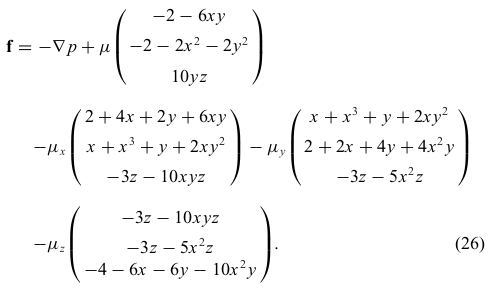
\includegraphics[width=8cm]{images/mms/busa13_eq26}
\end{center}
\end{remark}


%-----------------------------------
\subsection{Variable viscosity case}

The spatial derivatives of the viscosity are then given by
\begin{eqnarray}
\frac{\partial }{\partial x} \eta(x,y,z) &=& -(1-2x)\beta\; \eta(x,y,z) \nonumber\\
\frac{\partial }{\partial y} \eta(x,y,z) &=& -(1-2y)\beta\; \eta(x,y,z) \nonumber\\
\frac{\partial }{\partial z} \eta(x,y,z) &=& -(1-2z)\beta\; \eta(x,y,z) \nonumber
\end{eqnarray}
and the right-hand side by
\begin{eqnarray}
\vec{f} 
&=& 
-
\left(
\begin{array}{c}
yz+3x^2y^3z\\
xz +3x^3y^2z \\
xy+x^3y^3
\end{array}
\right)
+\eta
\left(
\begin{array}{c}
2+6xy  \\
2 + 2x^2 +  2y^2 \\
-10yz 
\end{array}
\right) 
-(1-2x)\beta \eta (x,y,z)
\left(
\begin{array}{c}
2\dot{\epsilon}_{xx} \\
2\dot{\epsilon}_{xy} \\
2\dot{\epsilon}_{xz} \\
\end{array}
\right) \\
&&
-(1-2y)\beta \eta (x,y,z)
\left(
\begin{array}{c}
2\dot{\epsilon}_{xy} \\
2\dot{\epsilon}_{yy} \\
2\dot{\epsilon}_{yz} \\
\end{array}
\right)
-(1-2z)\beta \eta (x,y,z)
\left(
\begin{array}{c}
2\dot{\epsilon}_{xz} \\
2\dot{\epsilon}_{yz} \\
2\dot{\epsilon}_{zz} \\
\end{array}
\right) \nonumber\\
&=& 
-
\left(
\begin{array}{c}
yz+3x^2y^3z\\
xz +3x^3y^2z \\
xy+x^3y^3
\end{array}
\right)
+\eta
\left(
\begin{array}{c}
2+6xy  \\
2 + 2x^2 +  2y^2 \\
-10yz 
\end{array}
\right) 
-
(1-2x)\beta \eta 
\left(
\begin{array}{c}
2+4x+2y+6x^2y \\
x+y+2xy^2+x^3 \\
-3z -10xyz 
\end{array}
\right) \nn \\
&&
-(1-2y)\beta \eta
\left(
\begin{array}{c}
x+y+2xy^2+x^3 \\
2+2x+4y+4x^2y \\
-3z-5x^2z \\
\end{array}
\right)
-(1-2z)\beta \eta
\left(
\begin{array}{c}
-3z -10xyz \\
-3z-5x^2z \\
-4-6x-6y-10x^2y
\end{array}
\right) \nonumber
\end{eqnarray}
which translates as follows in Python:
\begin{lstlisting}
def bx(x,y,z,beta):
    mu=np.exp(1-beta*(x*(1-x)+y*(1-y)+z*(1-z)) )
    mux=-beta*(1-2*x)*mu
    muy=-beta*(1-2*y)*mu
    muz=-beta*(1-2*z)*mu
    val=-(y*z+3*x**2*y**3*z) + mu * (2+6*x*y) \
        +(2+4*x+2*y+6*x**2*y) * mux \
        +(x+x**3+y+2*x*y**2 ) * muy \
        +(-3*z-10*x*y*z     ) * muz
    return val

def by(x,y,z,beta):
    mu=np.exp(1-beta*(x*(1-x)+y*(1-y)+z*(1-z)) )
    mux=-beta*(1-2*x)*mu
    muy=-beta*(1-2*y)*mu
    muz=-beta*(1-2*z)*mu
    val=-(x*z+3*x**3*y**2*z) + mu * (2 +2*x**2 + 2*y**2) \
       +(x+x**3+y+2*x*y**2   ) * mux \
       +(2+2*x+4*y+4*x**2*y  ) * muy \
       +(-3*z-5*x**2*z       ) * muz 
    return val

def bz(x,y,z,beta):
    mu=np.exp(1-beta*(x*(1-x)+y*(1-y)+z*(1-z)) )
    mux=-beta*(1-2*x)*mu
    muy=-beta*(1-2*y)*mu
    muz=-beta*(1-2*z)*mu
    val=-(x*y+x**3*y**3) + mu * (-10*y*z) \
       +(-3*z-10*x*y*z        ) * mux \
       +(-3*z-5*x**2*z        ) * muy \
       +(-4-6*x-6*y-10*x**2*y ) * muz 
    return val
\end{lstlisting}

%----------------------------------------
\subsection{root mean square velocity}

Let us now compute the root mean square velocity:
\begin{eqnarray}
\int_\Omega u^2 dx dy dz 
&=& \int_{0}^{+1}\int_{0}^{+1}\int_{0}^{+1} (x+x^2+xy+x^3y )^2 dx dy dz = 2867/1260 \nn \\
\int_\Omega v^2 dx dy dz 
&=& \int_{0}^{+1}\int_{0}^{+1}\int_{0}^{+1} (y + xy + y^2 + x^2 y^2 )^2 dx dy dz = 3947/1800 \nn  \\
\int_\Omega w^2 dx dy dz 
&=& \int_{0}^{+1}\int_{0}^{+1}\int_{0}^{+1} (-2z - 3xz - 3yz - 5x^2 yz )^2 dx dy dz = 463/36   \nn
\end{eqnarray}
then
\[
\upnu_{rms}=\sqrt{ 2867/1260 + 3947/1800 + 463/36  } \simeq 4.1628459
\]

